%
\section{Implementation}\label{sec:implementation}
This chapter explains how the component is developed. The ways to overcome the design challenges, some of the findings during the development have been written down.
%
\subsection{System Characteristics}
When beginning the implementation, I decided to use a simple yet powerful programming language for both frontend and backend applications to obtain my results. The programing languages which I selected was javascript for frontend and C\# for the backend. To simplify my programming work, I used the Visual Studio Code IDE for the frontend and Visual Studio 2019 for the backend. The configuration of the computer used for implementation is as follows:
\begin{description}
	\item [$\bullet$]Operating System: Windows 10 Enterprise 2016 - 64-bit
	\item [$\bullet$]Processor: Intel Core i7-6700 @ 3.4GHz
	\item [$\bullet$]RAM: 16GB
	\item [$\bullet$]HDD: 500GB
\end{description}

The software support tools used for frontend implementation are listed as follows:
\begin{description}
	\item [$\bullet$]Programming Language: Javascript
	\item [$\bullet$]IDE: Visual Studio Code
	\item [$\bullet$]Packet Manager: npm
	\item [$\bullet$]Version Control: Azure Repos
\end{description}

The software support tools used for backend implementation are listed as follows:
\begin{description}
	\item [$\bullet$]Programming Language: C\#
	\item [$\bullet$]IDE: Visual Studio 2019
	\item [$\bullet$]Packet Manager: NuGet
	\item [$\bullet$]Database: Azure Data Storage - Containers
	\item [$\bullet$]Version Control: Azure Repos
\end{description}

All the infrastructure and software that I used are provided by evosoft GmbH.
\subsection{OSS Component Analyzer}
The \acs{OSS} component analyzer is a starting point in the process of scanning the \acs{OSS} components from a project. This is a front-end module and it is implemented in the Angular framework using typescript language. The GUI interface of this module requires four inputs from the user which is project name, description, members and project source directory. It has two important tasks before it proceeds to the evaluation process. The first task, the module should find the required configuration file in the project. This configuration file identification was done with the help of a dependency manager. Each application framework has its own dependency manager and it generates a unique configuration file for the application framework. The below table shows all the config files of each application framework. The \acs{OSS} component names and versions will be listed in the config files. 
\begin{table}[h!]
\begin{center}
 \begin{tabular}{ |c|c|c|c| } 
 	\hline
 	Application Framework & Dependency Manager & Config file & File Type \\
 	\hline
 	.NET(Console Application) & Nuget & .csproj file & XML \\ 
 	Angular Framework & npm & package.json & JSON \\ 
 	Microsoft TFS & Nuget & app.config & XML \\ 
 	Django & npm & requirremen.txt & Text\\ 
 	Ruby on Rails & Rubygem & gemfile & File \\ 
 	Laravel & composer & composer.json & JSON \\ 
 	Gradle projects & gradle & build.gradle & GRADLE \\ 
 	Maven projects & POM & pom.xml & XML \\ 
 	.NET & Nuget & packages.config & XML \\ 
 	\hline
 \end{tabular}
\caption{Configuration file of each application framework.}\label{tab:configFiles}
\end{center} 
\end{table}

Once the respective config is identified from the project, the targeted data should be scrapped from config files. To achieve this, the automated scrapping methods are used based on the config file type. For instance the user is scanning Maven project, then according to the table the config file is a XML file so therefore to scrap the targeted data DOM parsing method is used. Likewise for \acs{JSON} file json parsing methods can be used, text pattern matching methods can be used for text file, Gemfile, FIle and GRADLE files. After scrapping the targeted data, the next task is to generate a json object with the project general information and scrapped \ac{OSS} information and will be ready to send it to the \acs{OSS} evaluation process. 
\newpage
 \begin{figure}[h!]
	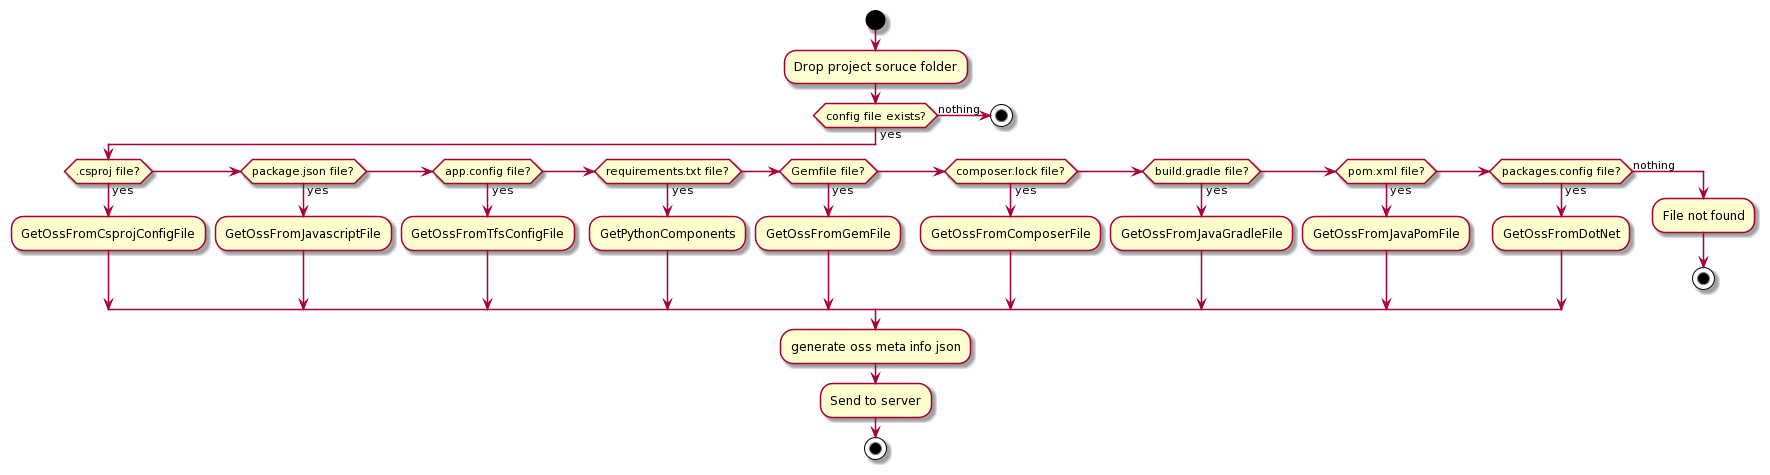
\includegraphics[width=15cm]{includes/OSS_Analyzer_Activity_Diagram.png}
	\centering
	\caption{\acs{OSS} Component Analyzer Activity Diagram}
	\label{fig:Analyzer_Activity_Diagram}
\end{figure}
\subsection{Component Evaluator}
The \acs{OSS} component evaluator is the final process of finding the vulnerabilities with the help of a vulnerability database. Once the server side application receives the json objects from the client application, the application will start searching the received components in the \acs{NVD} database. First component names and versions will be searched under the \acs{CPE} dictionary to verify the product has been registered in the \acs{CPE}. If the component is found in the \acs{CPE} dictionary, the service returns all the results of the component name. To verify the component name and the version is not a regular process because the \acs{CPE} name has its own naming specification. The figure ~\ref{fig:cpe_name} is an example of the \acs{CPE} naming specification.
 \begin{figure}[h!]
	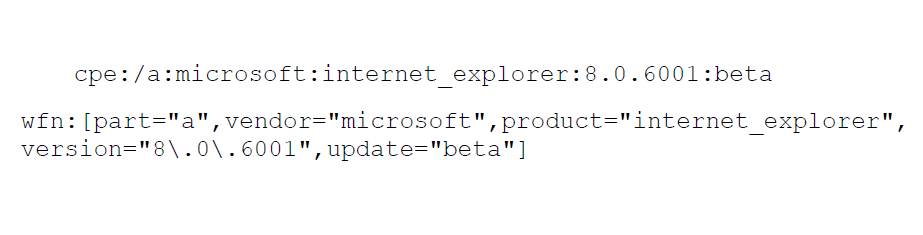
\includegraphics[width=15cm]{includes/cpe_name.png}
	\centering
	\caption{CPE name specification}
	\label{fig:cpe_name}
\end{figure}
From the figure ~\ref{fig:cpe_name} it is visible that the component name and version are in the 3rd and 4th position of the \acs{CPE} string. The given component name and version must be verified with the \acs{CPE} name. As the second stage of verification, the given component name and \acs{CPE} name is verified again by using the Hamming distance algorithm. By having this second stage of verification it can make sure the component is legit. Once the \acs{CPE} name is validated with the given component, the next step will be retrieving the \acs{CVE} details using the \acs{CPE} name to find out the vulnerability information. \acs{CVE} retrieval API services are used to find the vulnerability information. After retrieving the relevant vulnerability information of the component, the entire project information will be created as a \acs{JSON} object and will be stored as a container in the Azure data storage.
\newpage 
\begin{figure}[h!]
	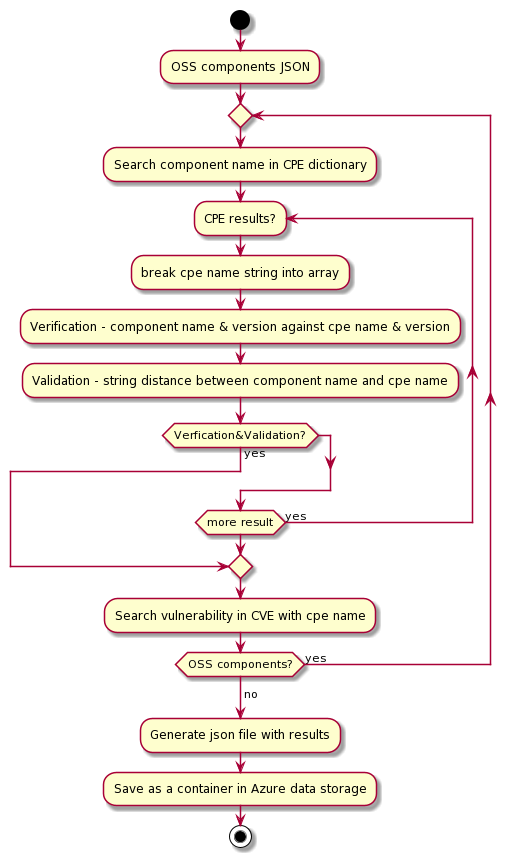
\includegraphics[width=15cm,height=20cm]{includes/OSS_Evaluator_Activity_Diagram.png}
	\centering
	\caption{\acs{OSS} Component Evaluator Activity Diagram}
	\label{fig:Evaluator_Activity_Diagram}
\end{figure} 
\newpage                                                                                      \newpage            
\subsection{Reporter}
The Reporter is the final module of the \acs{OSS} scanner and it is implemented in the client side of the application. This module is implemented in the Angular framework by using the jspdf library. The main purpose of this module is to generate a report of the scanned projects by containing the \acs{CVSS} information of each \acs{OSS} component. The report will consist only of the necessary and human understandable information in the report so this makes the user have a clear understanding of the report and also helps to make decision. The information for the report will be retrieved from the Azure data storage whereas an \acs{API} service has been developed in the backend system to retrieve the project information from the Azure data storage.
%
\begin{figure}[h!]
	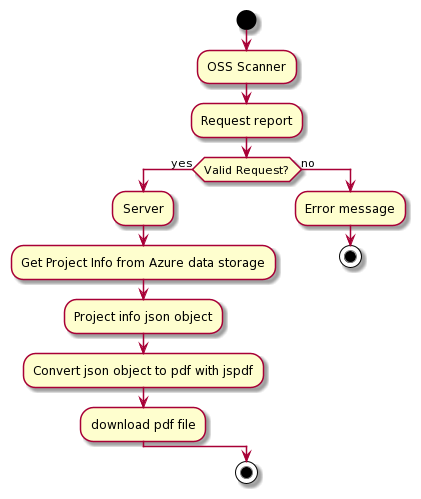
\includegraphics[width=15cm]{includes/Reporter_Activity_Diagram.png}
	\centering
	\caption{\acs{OSS} Component Evaluator Activity Diagram}
	\label{fig:Reporter_Activity_Diagram}
\end{figure}   